\section{Support Vector Machine}

\subsection{Optimization Objective}
    \subsubsection{Alternative View of Logistic Regression}
        \[
            h_\theta(x) = \frac{1}{1 + e^{-\theta^T x}} 
        \] 

        If y = 1, we want $h_\theta(x) \approx 1$, $\theta^T x >> 0$. 
        \par If y = 0, we want $h_\theta(x) \approx 0$, $\theta^T x << 0$
        
        Cost of example:
        \[
            \boxed{
        y\;log\;h_\theta(x)\:\;+\:\;(1-y)\;log(1-h_\theta(x)))\;=\;-y\;log\;\frac{1}{1\;+\;e^{-\theta^Tx}}\;-\;(1-y)\;log\;(1-\frac{1}{1+\;e^{\theta^T\;x}})
            }
        \] 

        Consider the two terms in the above equation, where now we replace the cost with a straightened two-section curve:
 
        \begin{figure}[htbp]
            \centering
            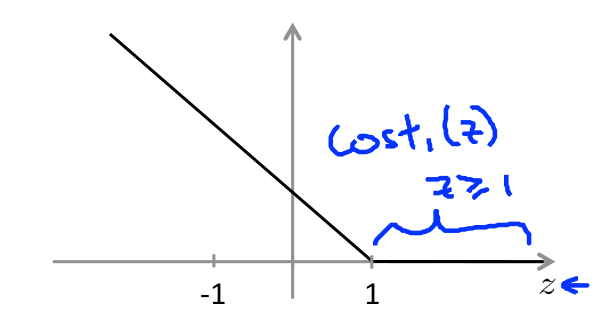
\includegraphics[width=0.5\textwidth]{image/SVM-cost1.png}
            \caption{SVM cost\textsubscript{1}}
            \label{fig:SVM-cost1}
        \end{figure}

       \begin{figure}[htbp]
            \centering
            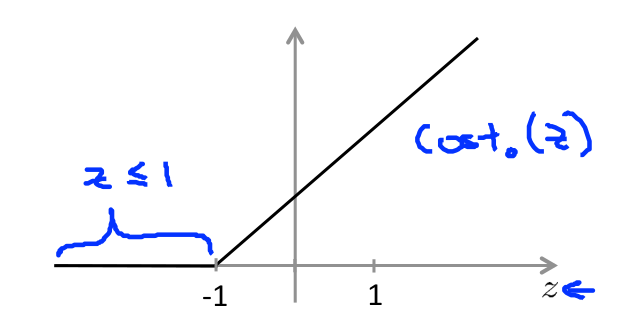
\includegraphics[width=0.5\textwidth]{image/SVM-cost0.png}
            \caption{SVM cost\textsubscript{0}}
            \label{fig:SVM-cost0}
        \end{figure}

        \begin{enumerate}
            \item If y=1 , want $h_\theta(x) \approx 1$, $\theta^T x >> 0$. Here we label the curve as cost\textsubscript{0} (z), as shown in Figure \ref{fig:SVM-cost1}.
            \item If y = 0, we want $h_\theta(x) \approx 0$, $\theta^T x << 0$. Here we label the curve as cost\textsubscript{1}(z), as shown in Figure \ref{fig:SVM-cost0}..
        \end{enumerate}

        \subsubsection{Support Vector Machine}
        Recall logistic regression has the form as in Equation \ref{eq:logistic-cost-function-regularized}, shown below in an alternate form (taking the negative sign into the summation):
    \[
J(\theta) = \frac{1}{m} \, \sum_{i=1}^{m}\, [ y^{(i)}\, -log\, h_\theta (x^{(i)})\; \; -(1-y^{(i)})\: log\:(\,1-h_\theta(x^{(i)})\,) ] + \frac{\lambda}{2m} \sum_{j=1}^{n} \theta_j^2
    \] 

    The Support Vector Machine has a similar form as logistic regression, with a few conventions that differ from its logistic regression counterpart:
    \begin{enumerate}
        \item Remove scaling term ($\frac{1}{m}$). Note that this does not change the final result of minimized $\theta$.
        \item The logistic regression has the form: $A + \lambda B$; the SVM has the form $CA + B$. This is just a different way of parametrizing tradeoffs. Note here C behaves similarly to $\frac{1}{\lambda}$.
    \end{enumerate}

    Therefore, the SVM hypothesis can be expressed in Equation \ref{eq:svm}.

    \begin{equation}
        \underset{\theta}{min}\: C \sum_{i=1}^{m}\, [ y^{(i)}\, cost_1 (\theta^T x^{(i)}) + \; (1-y^{(i)})\:cost_0 (\theta^T x^{(i)})] + \frac{1}{2} \sum_{j=1}^{n} \theta_j^2
        \label{eq:svm}
    \end{equation}

    The hypothesis
    \[
        h_\theta (x) = 
        \begin{cases}
       1 &\quad \text{if } \theta^T x \geq 0 \\
       0 &\quad \text{if otherwise. }  \\
        \end{cases}
    \]

\subsection{Large Margin Intuition}
Recall in Figure \ref{fig:SVM-cost1} and \ref{fig:SVM-cost0}, we re-defined the function. Herein, we have shifted our threshold to z=1 and z=-1 respectively for predicting y = 1 and 0, respectively. This is different from previous threshold of 0 for logistic regression. We are more conservative in our predictions here, by using the 2 new segment cost functions, cost\textsubscript{1}($\theta^T x^{(i)}$) and cost\textsubscript{0}($\theta^T x^{(i)}$). 
    \subsubsection{SVM Decision Boundary}
    Suppose we set C to be a large number, e.g. 10000. Under the minimization objective, we will be highly motivated to pick a $\theta$ such that the first term is close to zero, thus discarding the first term. 
    The original equation will then be reduced effectively to 
    \[
        \underset{\theta}{min} \: \frac{1}{2} \sum_{j=1}^{n} \theta_j^2
    \] 
    
    such that 
    \[
    \theta^T x^{(i)}
         \begin{cases}
       \geq 1 &\quad \text{if } y^{(i)} = 1\\
       \leq -1 &\quad \text{if } y^{(i)} = 0  \\
        \end{cases}
    \] 

    \subsubsection{Large Margin Classifier}
    The Support Vector Machine is also known as the Large Margin Classifier. The word margin refers to the distance between the boundary and the data points. SVM will try to maximize the distance, as seen in Figure \ref{fig:SVM-decision-boundary-margin}. 
    \begin{figure}[htbp]
        \centering
        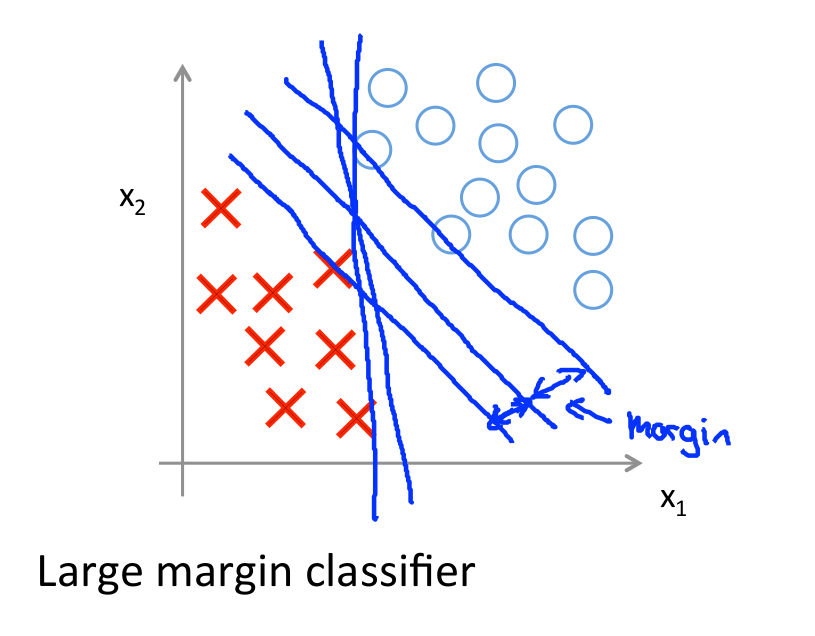
\includegraphics[width=0.5\textwidth]{image/SVM-decision-boundary-margin.png}
        \caption{SVM Decision Boundary: Linearly Separable Case}
        \label{fig:SVM-decision-boundary-margin}
    \end{figure}

        When C is too large (similar to a small $\lambda$), then we get decrease the power of the margin margin classifier, and the algorithm will fit too well to outliers. 

\subsection{Kernels}
    \subsubsection{Non-linear decision boundary}
    For a non-linear decision boundary problem (as shown in Figure \ref{fig:non-linear-decision-boundary-problem}), we have:
        \[
            h_{\theta} = 
            \begin{cases}
                1,                      &\quad \text{if } \theta_0 x + \theta_1 x_1 + \dots \geq 0 \\
                0,                      &\quad \text{otherwise } \\
            \end{cases}
        \] 

        This can be written as 
        \[
        \theta_0 x + \theta_1 f_1 + \theta_2 f_2+ \theta_3 f_3 + \dots
        \] 
        , where 
        \[
            f_1 = x_1, f_2 = x_2, f_3 = x_1x_2, f_4 = x_1^2, f_5 = x_2^2 \dots
        \] 


        However, high order polynomials are expensive. Is there a better choice of features $f_i$'s?

        \begin{figure}[htpb]
            \centering
            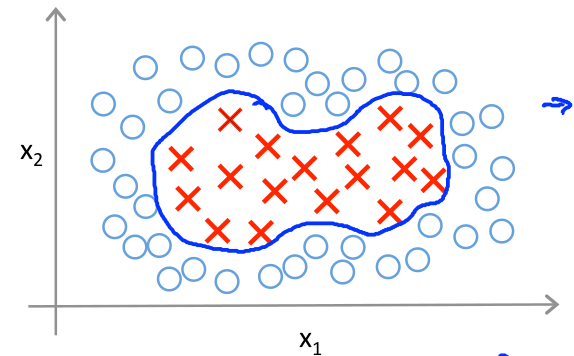
\includegraphics[width=0.5\textwidth]{image/non-linear-decision-boundary.png}
            \caption{Nonlinear decision boundary problem}
            \label{fig:non-linear-decision-boundary-problem}
        \end{figure}

    \subsubsection{Kernel}
    Given $x$, compute new feature depending on proximity to landmarks $l^{(1)}, l^{(2)}, l^{(3)}$. This can be illustrated in Figure \ref{fig:landmark}. 

    \begin{figure}[htbp]
        \centering
        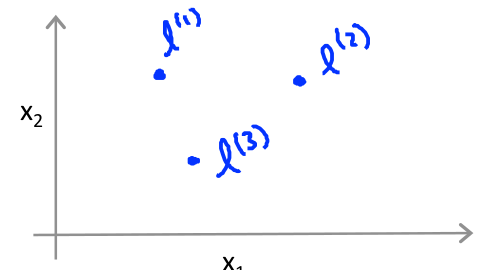
\includegraphics[width=0.5\textwidth]{image/landmark.png}
        \caption{Kernel and landmark illustration}
        \label{fig:landmark}
    \end{figure}

    We then compute the features $f_i = kernel(x, l^{(i)})$ as follows: 
    \begin{equation}
        f_i = \text{similarity}(x, l^{(i)}) = exp ( - \frac{\| x-l^{(i)}\|^2}{2\sigma^2})
        \label{eq:guassian-kernel}
    \end{equation}
    This is a specific type of kernel, namely, the \emph{Gaussian kernel}.

    \subsubsection{Kernels and Similarity} 
    Note: The term $\| x-l^{(i)} \|$ in \ref{eq:guassian-kernel} can also be written as: $\sum_{j=1}^{n} (x^j - l^{(i)}_j)^2$. We can analyze the term in two scenarios:
    \begin{enumerate}
        \item If $x\approx l^{(i)}$, then $\| x-l^{(i)} \|\approx 0$, consequently $f_i \approx 1$.
        \item If $x$ is far from $l^{(i)}$, then $\| x-l^{(i)} \|$ large, consequently $f_i \approx 0$.
    \end{enumerate}

    Each landmark $l^{(i)}$ defines a new feature $f_i$, where the function approaches one when x is close to the landmark, and approaches zero otherwise.

    The function can be visualized in Figure \ref{fig:guassian-kernel-plot}. Note that as the variance ($\sigma$) increases, f falls from the peak (1) slower.
   \begin{figure}[htpb]
       \centering
       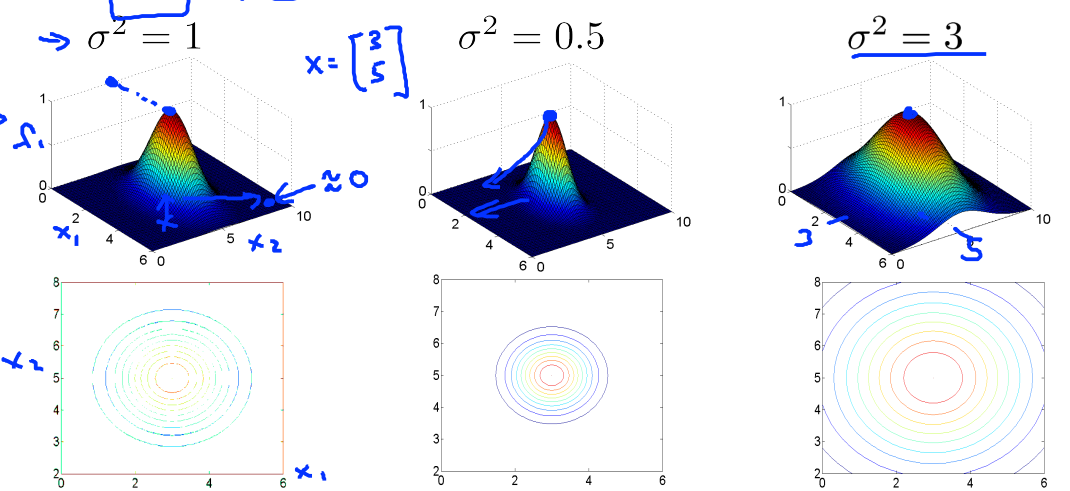
\includegraphics[width=0.7\textwidth]{image/guassian-kernel-plot.png}
       \caption{Guassian Kernel 3D plot}
       \label{fig:guassian-kernel-plot}
   \end{figure} 
   \subsubsection{Choosing Landmark}
   A natural question arises: \emph{Where do we get $l^{(i)}$?} 
   \par Recall from \ref{eq:guassian-kernel}, given x we can compute a feature (f\textsubscript{i}) as the similarity between the point and the landmark.   


   We predict y = 1, when 
   \[
       \sum_{i}^{n} \theta_i f_i \geq 0
   \] 
   In practise, $\theta_0$ is chosen to be negative, where $\theta_i, (i\neq 0)$ are chosen to be some non-negative constants. As such, the closer $x_i$ is to each $l_i$, $f_i$ will tend to 1, thus making the term $\theta_i f_i$ some positive number. We then take the sum of "weighted proximities to each landmark", and make the decision on y. 

   \par Observe Figure \ref{fig:landmark-selection}, where the markings of datasets we want is in blue, and red are the ones that we discard. Our goal is to guess what data belongs to our identification. Hence, we want to identify $x$ that is close to our training examples. 

   \begin{figure}[htpb]
       \centering
       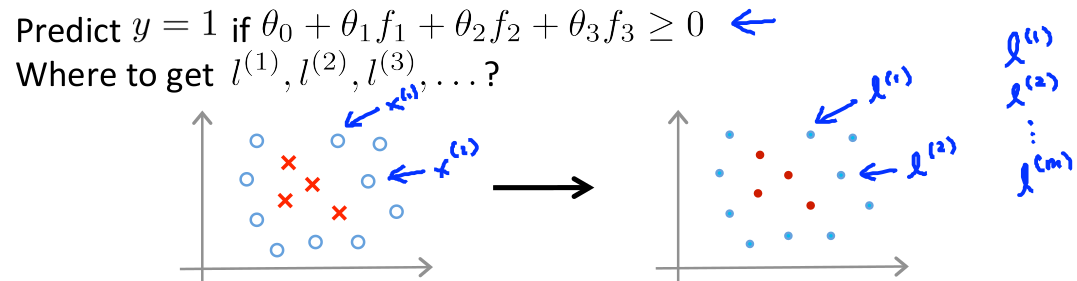
\includegraphics[width=0.7\textwidth]{image/landmark-selection.png}
       \caption{Landmark and Training dataset}
       \label{fig:landmark-selection}
   \end{figure}

   \par Comparing the above two paragraphs, it follows naturally that we should choose the training examples as our landmarks. Thus features are a measure of \emph{proximity to training examples}, given an $x$.
   \subsubsection{SVM with Kernels}
        A summary of our setup:
        \begin{itemize}
            \item Given training examples:  $(x^{(i)}, y^{(i)})$, i = $1\dots m$.
            \item Select landmarks:         $l^{(i)} = x^{(i)}$
            \item Given example $x$:   compute features $f_i = similarity(x, l^{(i)})$. \\
                For training example $(x^{(i)}, y^{(i)})$, where $x^{(i)} \in \mathbb{R}^{n+1} \; (0 \dots n)$. We can compute the feature vector $f^{(i)} \in \mathbb{R}^{m+1}$, where $m$ is the number of landmarks (training examples).
                \[
                f^{(i)} = \begin{bmatrix}
                    f_0^{(i)}   \\
                    f_1^{(i)}   \\
                    f_2^{(i)}   \\
                    \vdots      \\
                    f_i^{(i)}   \\
                    \vdots      \\
                    f_m^{(i)}
                            \end{bmatrix}
                \] 
                \begin{enumerate}
                    \item $f_0^{(i)} = 1$ by default.
                    \item $f_i^{(i)} = 1$ by design (check Equation \ref{eq:guassian-kernel}; similarity of $x^{(i)}$ to $l^{(i)}= x^{(i)}$ is 1).
                \end{enumerate}
                    
        \end{itemize}


        Formally:
        \begin{enumerate}
            \item \textbf{Hypothesis}: Given $x \in \mathbb{R}^{n+1}$, compute features $f \in \mathbb{R}^{m+1}$. \\
                Predict "y = 1", if $\theta^T f  = \sum_{i=0}^{m} \theta_i f_i \geq 0$
            \item \textbf{Training}: 
                \[
        \underset{\theta}{min}\: C \sum_{i=1}^{m}\, [ y^{(i)}\, cost_1 (\theta^T f^{(i)}) + \; (1-y^{(i)})\:cost_0 (\theta^T f^{(i)})] + \frac{1}{2} \sum_{j=1}^{m} \theta_j^2
            \] 
                Remarks: 
                \begin{itemize}
                    \item The above equation is similar to \ref{eq:svm}.
                    \item We calculate the cost based on $\theta$ and $f^{i}$.
                    \item In the second summation, $n=m$; number of features=number of training sets.
                \end{itemize}
            \item \textbf{Implementation Note}
                \begin{itemize}
                    \item $\sum_{j=1}^{m} \theta_j^2 = \theta^T \theta; 
                            \theta = \begin{bmatrix}
                            f_0     \\
                            f_1     \\
                            f_2     \\
                            \vdots  \\
                            f_m     \\
                                    \end{bmatrix}$ 
                    \item Can also scale $\theta$, i.e. $\theta^T M \theta$.
                    \item $M$ increases computation efficiency.
                \end{itemize}
        \end{enumerate}

        
    \subsubsection{SVM Parameters}
    We have two parameters: C and $\lambda$: \\
    \par \textbf{C}= $\frac{1}{\lambda}$:
    \begin{enumerate}
        \item Large C (small $\lambda$): lower bias, higher variance.
        \item Small C (large $\lambda$): Higher bias, low variance.
    \end{enumerate}

    \par \textbf{$\sigma^2$}: (see Figure \ref{fig:guassian-kernel-plot})
    \begin{enumerate}
        \item Large $\sigma^2$: (features $f_i$ vary more smoothly) higher bias, lower variance.
        \item Small $\sigma^2$: (changes abruptly) lower bias, higher variance.
    \end{enumerate}

